% figures/latency-by-bucket.tex — outline-emission latency by LoC bucket.
% Data: data/aggregated/outline-latency.csv (cols warm_p50_ms, warm_p95_ms).
% Backs §6.4 (OQ-AST-2). Go files only (Phase 1a).
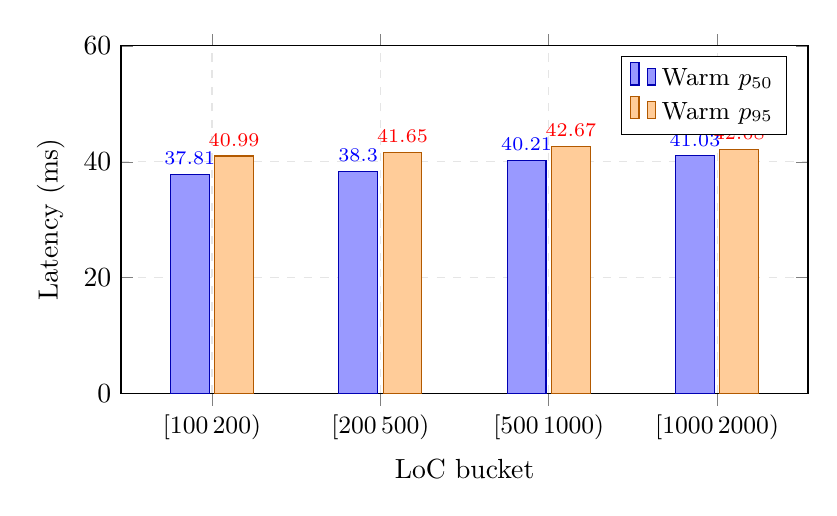
\begin{tikzpicture}
\begin{axis}[
    width=0.85\textwidth,
    height=6cm,
    ybar,
    bar width=14pt,
    ymin=0, ymax=60,
    enlarge x limits=0.18,
    ylabel={Latency (ms)},
    xlabel={LoC bucket},
    symbolic x coords={[100\,200), [200\,500), [500\,1000), [1000\,2000)},
    xtick=data,
    xticklabel style={font=\small},
    nodes near coords,
    nodes near coords align={vertical},
    nodes near coords style={font=\scriptsize},
    grid=major,
    grid style={dashed,gray!20},
    legend style={at={(0.97,0.97)}, anchor=north east, font=\small},
]
% warm_p50_ms — median of warm runs across files per bucket
% Values from data/aggregated/outline-latency.csv (Go, Phase 1a)
\addplot+[fill=blue!40, draw=blue!70!black] coordinates {
  ([100\,200),  37.81)
  ([200\,500),  38.30)
  ([500\,1000), 40.21)
  ([1000\,2000), 41.03)
};
% warm_p95_ms — 95th-percentile of warm runs across files per bucket
\addplot+[fill=orange!40, draw=orange!70!black] coordinates {
  ([100\,200),  40.99)
  ([200\,500),  41.65)
  ([500\,1000), 42.67)
  ([1000\,2000), 42.08)
};
\legend{Warm $p_{50}$, Warm $p_{95}$}
\end{axis}
\end{tikzpicture}
